% Created 2018-04-09 lun 18:26
% Intended LaTeX compiler: pdflatex
\documentclass[xcolor={usenames,svgnames,dvipsnames}]{beamer}
\usepackage[utf8]{inputenc}
\usepackage[T1]{fontenc}
\usepackage{graphicx}
\usepackage{grffile}
\usepackage{longtable}
\usepackage{wrapfig}
\usepackage{rotating}
\usepackage[normalem]{ulem}
\usepackage{amsmath}
\usepackage{textcomp}
\usepackage{amssymb}
\usepackage{capt-of}
\usepackage{hyperref}
\usepackage{color}
\usepackage{listings}
\usepackage{mathpazo}
\usepackage{gensymb}
\usepackage{amsmath}
\usepackage{chemarr}%flechas para reacciones químicas (SFER.tex)
\bibliographystyle{plain}
\AtBeginSubsection[]{\begin{frame}[plain]\tableofcontents[currentsubsection,sectionstyle=show/shaded,subsectionstyle=show/shaded/hide]\end{frame}}
\AtBeginSection[]{\begin{frame}[plain]\tableofcontents[currentsection,hideallsubsections]\end{frame}}
\usepackage[emulate=units]{siunitx}
\sisetup{fraction=nice, decimalsymbol=comma, retain-unity-mantissa = false}
\newunit{\wattpeak}{Wp}
\newunit{\watthour}{Wh}
\newunit{\amperehour}{Ah}
\hypersetup{colorlinks=true, linkcolor=Blue, urlcolor=Blue}
\renewcommand{\thefootnote}{\fnsymbol{footnote}}
\beamertemplatenavigationsymbolsempty
\setbeamertemplate{footline}[frame number]
\setbeamercolor{alerted text}{fg=blue!50!black} \setbeamerfont{alerted text}{series=\bfseries}
\usetheme[hideothersubsections]{Goettingen}
\usecolortheme{rose}
\usefonttheme{serif}
\author{Oscar Perpiñán Lamigueiro \\ \url{http://oscarperpinan.github.io}}
\date{}
\title{Sistemas Fotovoltaicos Autónomos}
\subtitle{Diseño}
\hypersetup{
 pdfauthor={Oscar Perpiñán Lamigueiro \\ \url{http://oscarperpinan.github.io}},
 pdftitle={Sistemas Fotovoltaicos Autónomos},
 pdfkeywords={},
 pdfsubject={},
 pdfcreator={Emacs 25.2.2 (Org mode 9.1.9)}, 
 pdflang={Spanish}}
\begin{document}

\maketitle

\section{Dimensionado del SFA}
\label{sec:org5d06901}
\begin{frame}[label={sec:orgceca8b9}]{Objetivo}
\begin{itemize}
\item El dimensionado de un SFA consiste en \alert{decidir el tamaño del
generador fotovoltaico y acumulador} que serán capaces de
\alert{proporcionar la energía requerida} por una determinada carga a partir
de la \alert{radiación disponible} en la zona.

\item Debido al comportamiento aleatorio tanto de la radiación como del
consumo, la \alert{probabilidad de fallo no es nula}.

\item La solución es un compromiso entre el coste y la fiabilidad del
sistema.
\end{itemize}
\end{frame}


\subsection{Nomenclatura}
\label{sec:org0effe48}
\begin{frame}[label={sec:org57c246b}]{Carga}
\begin{description}
\item[{Consumo:}] \(L\)

\item[{Probabilidad de pérdida de carga:}] relación entre la energía que no
puede suministrar el sistema fotovoltaico y la energía solicitada por
la carga durante todo el período de
funcionamiento.$$LLP=\frac{E_{def}}{L}$$
\end{description}
\end{frame}

\begin{frame}[label={sec:org2ec6f2e}]{Capacidades normalizadas}
\begin{description}
\item[{Capacidad del generador:}] relación entre los valores medios de la
energía que puede producir el generador y la energía consumida por la
carga.
$$C_{A}=\frac{\eta_{G}\cdot A_{G}\cdot\overline{G_{d}}(\beta,\alpha)}{L}$$

\item[{Capacidad de acumulación:}] relación entre la capacidad útil del acumulador y la energía consumida por la carga.
\end{description}
$$C_{s}=\frac{C_{U}}{L}=\frac{C_{B}\cdot PD_{max}}{L}$$
\end{frame}

\subsection{Objetivo}
\label{sec:org2d2415d}
\begin{frame}[label={sec:org3a4ba04}]{Dimensionado}
\begin{block}{La tarea de dimensionar un sistema fotovoltaico consiste en encontrar la mejor solución de compromiso entre coste y fiabilidad.}
\begin{itemize}
\item Diferentes valores de \((C_{A},\, C_{S})\) pueden conducir al mismo
valor de \(LLP\).

\item Cuanto mayor es el sistema, mayor es la fiabilidad, pero mayor es el
coste.
\end{itemize}
\end{block}
\end{frame}


\subsection{Ejemplos}
\label{sec:org323c0b7}
\begin{frame}[label={sec:org9c78e01}]{Generador grande, acumulador pequeño}
\begin{itemize}
\item La \alert{combinación de \(C_{A}\) alta y \(C_{S}\) baja} conduce a ciclados
diarios con descargas profundas y ciclados estacionales
cortos.

\begin{itemize}
\item Las descargas profundas y frecuentes son perjudiciales para la
batería,

\item La corta longitud de los ciclados estacionales es beneficiosa.

\item La estratificación será fácilmente compensable con sobrecargas
controladas aplicando el mantenimiento adecuado.
\end{itemize}
\end{itemize}
\end{frame}

\begin{frame}[label={sec:orgf37cd9c}]{Generador pequeño, acumulador grande}
\begin{itemize}
\item La \alert{combinación de \(C_{A}\) baja y \(C_{S}\) alta} conduce a ciclados
diarios con descargas moderadas y ciclados estacionales largos.

\begin{itemize}
\item La baja profundidad de descarga es beneficiosa para la batería,

\item La longitud de los ciclados estacionales puede favorecer la
sulfatación y la estratificación.

\item Dado el tamaño relativo del generador frente al acumulador, la
frecuencia de sobrecargas será baja y la estratificación no será
tan fácilmente compensada.
\end{itemize}
\end{itemize}
\end{frame}

\begin{frame}[label={sec:org7b2f46b}]{Sistemas Híbridos}
\begin{itemize}
\item Cuando \(LLP\) es muy alta (p.e. radioenlaces) o la demanda es muy
elevada (poblados) el generador y acumulador serán excesivamente
grandes.

\item Es habitual incluir un grupo electrógeno que suministra la energía
deficitaria y permite reducir el tamaño del SFA.

\item Sinergia:

\begin{itemize}
\item El grupo electrógeno reduce el tamaño del generador FV y el
acumulador sin reducir fiabilidad.

\item El generador fotovoltaico reduce horas de funcionamiento del
grupo: gasto en combustible y mantenimiento.
\end{itemize}
\end{itemize}
\end{frame}

\subsection{Métodos de dimensionado}
\label{sec:org0a2b559}
\begin{frame}[label={sec:orge5d688b}]{Métodos de dimensionado}
\begin{block}{Método del LLP}
A partir de simulaciones o de curvas de isofiabilidad, establece los
valores de \(C_{A}\) y \(C_{S}\) para un consumo determinado.
\end{block}

\begin{block}{Método del mes peor}
\begin{itemize}
\item Determina el tamaño de batería y generador para abastecer el consumo durante el mes con peor relación entre radiación y consumo.
\item Si el consumo es constante, el mes peor es aquel de menor radiación.
\item Recomendaciones de expertos según zona geográfica y aplicación (tipología de consumo).
\end{itemize}
\end{block}
\end{frame}

\begin{frame}[label={sec:org147d2b0}]{Método del LLP}
\begin{center}
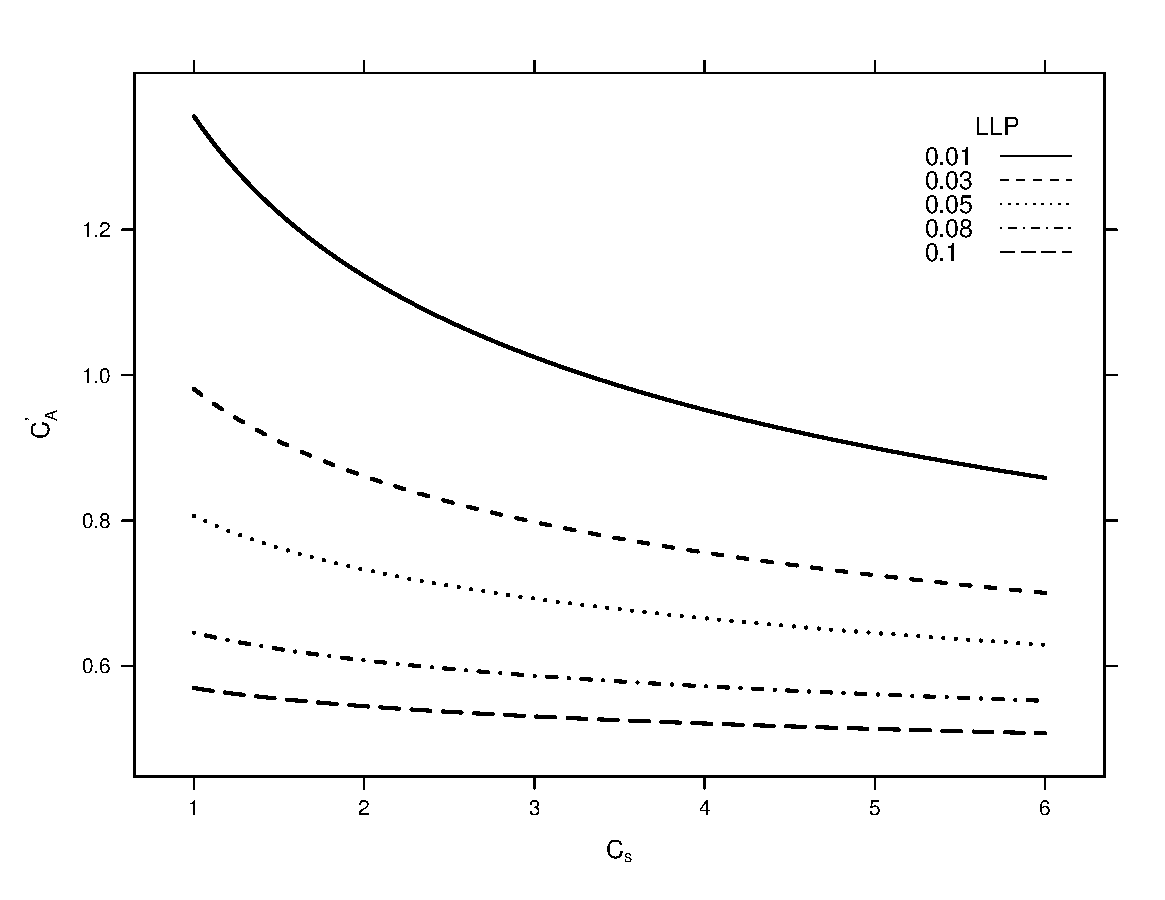
\includegraphics[width=.9\linewidth]{../figs/CurvasLLP.pdf}
\end{center}
\end{frame}

\begin{frame}[label={sec:org75bc169}]{Relación entre tamaño de generador y LLP}
\begin{itemize}
\item \(C_{s}=3\)
\end{itemize}

\begin{center}
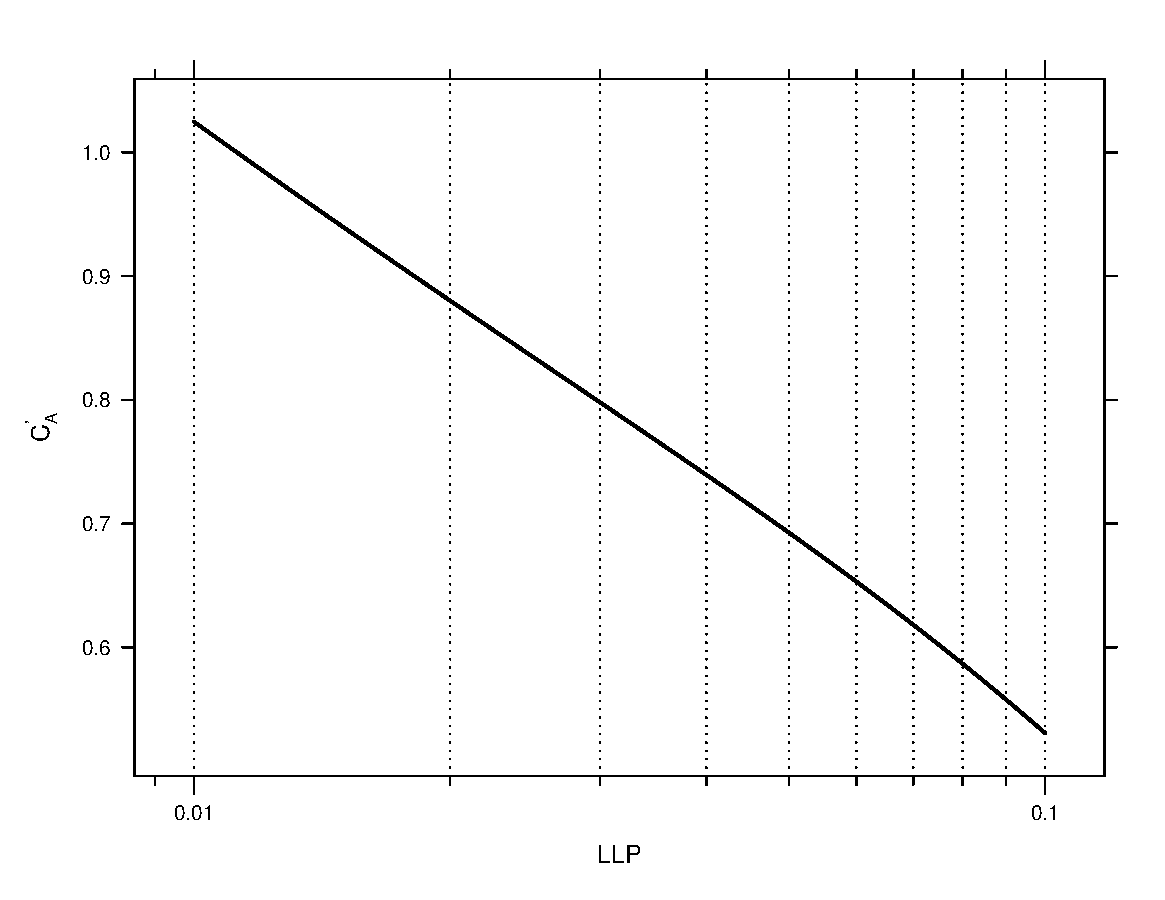
\includegraphics[width=.9\linewidth]{../figs/CurvasLLP_Cs3.pdf}
\end{center}
\end{frame}

\begin{frame}[label={sec:orgf700976}]{Método de LLP}
\begin{itemize}
\item Este proceso de cálculo se apoya en series de valores de radiación
solar que reproducen el comportamiento estadístico de la
irradiación.

\item La predicción del comportamiento del sistema limitada por la
incertidumbre asociada.

\item Los ejercicios de cálculo para probabilidades de pérdida de carga
inferiores a \(LLP=\num{1e-2}\) carecen de utilidad.
\end{itemize}

\begin{block}{Recordatorio}
\guillemotleft{}[\ldots{}] los modelos de simulación muy exactos pueden proporcionar números también muy exactos, pero ello no significa que se traduzcan automáticamente en predicciones también muy exactas.\guillemotright{}
\end{block}
\end{frame}

\begin{frame}[label={sec:orge079e9b}]{Método del mes peor}
\begin{block}{Valores según el UTS for SHS}
\begin{itemize}
\item Electrificación rural:

\begin{itemize}
\item \(C_{A}=1.1\)

\item \(3\leq C_{S}\leq5\)
\end{itemize}

\item Aplicaciones profesionales:

\begin{itemize}
\item \(1.2\leq C_{A}\leq1.3\)

\item \(5\leq C_{S}\leq8\)
\end{itemize}
\end{itemize}
\end{block}
\end{frame}

\subsection{Configuración de generador y batería}
\label{sec:org0989d62}
\begin{frame}[label={sec:org8b44350}]{Configuración de generador y batería}
\begin{itemize}
\item Una vez elegidos los valores de \(C_{A}\) y \(C_{S}\), se deben
configurar el generador y batería de acuerdo a las tensiones de
trabajo.

\item En general, la batería impone la tensión de trabajo (no hay buscador
de MPP). Supondremos \(V_{mpp} \simeq V_{b}\)

\item Carga en Ah
\end{itemize}
\[
Q_L = L / V_b
\]
\end{frame}

\begin{frame}[label={sec:orge0a3890}]{Batería}
\begin{itemize}
\item Capacidad en Ah (es recomendable no usar baterías en paralelo)
\end{itemize}
\[
Q_B = \frac{C_S \cdot Q_L}{PD}
\]

\begin{itemize}
\item Hay que elegir el número de vasos en serie adecuados a \(V_b\)
\end{itemize}
\end{frame}


\begin{frame}[label={sec:org425aec1}]{Generador}
\begin{itemize}
\item Capacidad del generador
\end{itemize}
\[
C_{A} = \frac{\eta_{G}\cdot A_{G}\cdot\overline{G_{d}}(\beta,\alpha)}{Q_L \cdot V_b}
\]


\begin{itemize}
\item Corriente de funcionamiento (determina número de ramas)
\end{itemize}

\begin{align*}
I_{g}^{*}\cdot V_{b} &= \eta_{G}\cdot A_{G}\cdot G_{stc}\\
I_{g}^{*} &=  \frac{C_{A}\cdot Q_{L}\cdot G_{stc}}{\overline{G_{d}}(\beta,\alpha)}
\end{align*}

\begin{itemize}
\item Hay que elegir el número de módulos en serie adecuados a \(V_b\)
\end{itemize}
\end{frame}

\begin{frame}[label={sec:org17f1579}]{Inclinación del generador}
\begin{itemize}
\item Para instalaciones con \alert{consumos constantes o similares a lo largo del año}, se busca maximizar la radiación en los meses de menor insolación $$\beta=|\phi|+10^{\circ}$$

\item Para instalaciones con \alert{consumo menor en meses de baja radiación} se busca maximizar radiación en equinoccios.$$\beta=|\phi|$$

\item Para instalaciones con \alert{uso predominante en verano} (hemisferio Norte) conviene emplear un ángulo inferior a la latitud. $$\beta=|\phi|-10^{\circ}$$

\item En general, la inclinación \alert{debe superar} los \(15^{\circ}\).
\end{itemize}
\end{frame}

\section{Consumo}
\label{sec:orgcba67d2}

\subsection{Estimación del consumo}
\label{sec:org9ea9d8c}
\begin{frame}[label={sec:org20166e5}]{Cálculo del consumo}
\begin{itemize}
\item Energía total requerida por las cargas
\end{itemize}
$$L_{T}=\frac{L_{dc}}{\eta_{r}}+\frac{L_{ac}}{\eta_{inv}}$$

\begin{itemize}
\item Energía producida por el generador
\end{itemize}
$$L=\frac{L_{T}}{\eta_{bat}\cdot\eta_{c}}$$

Como valores orientativos pueden utilizarse

\(\eta_{inv}=0.9\), \(\eta_{r}=0.95\), \(\eta_{bat}=0.85\) y \(\eta_{c}=0.98\).
\end{frame}

\begin{frame}[label={sec:org7a6ad2c}]{Distribución del consumo}
\begin{center}
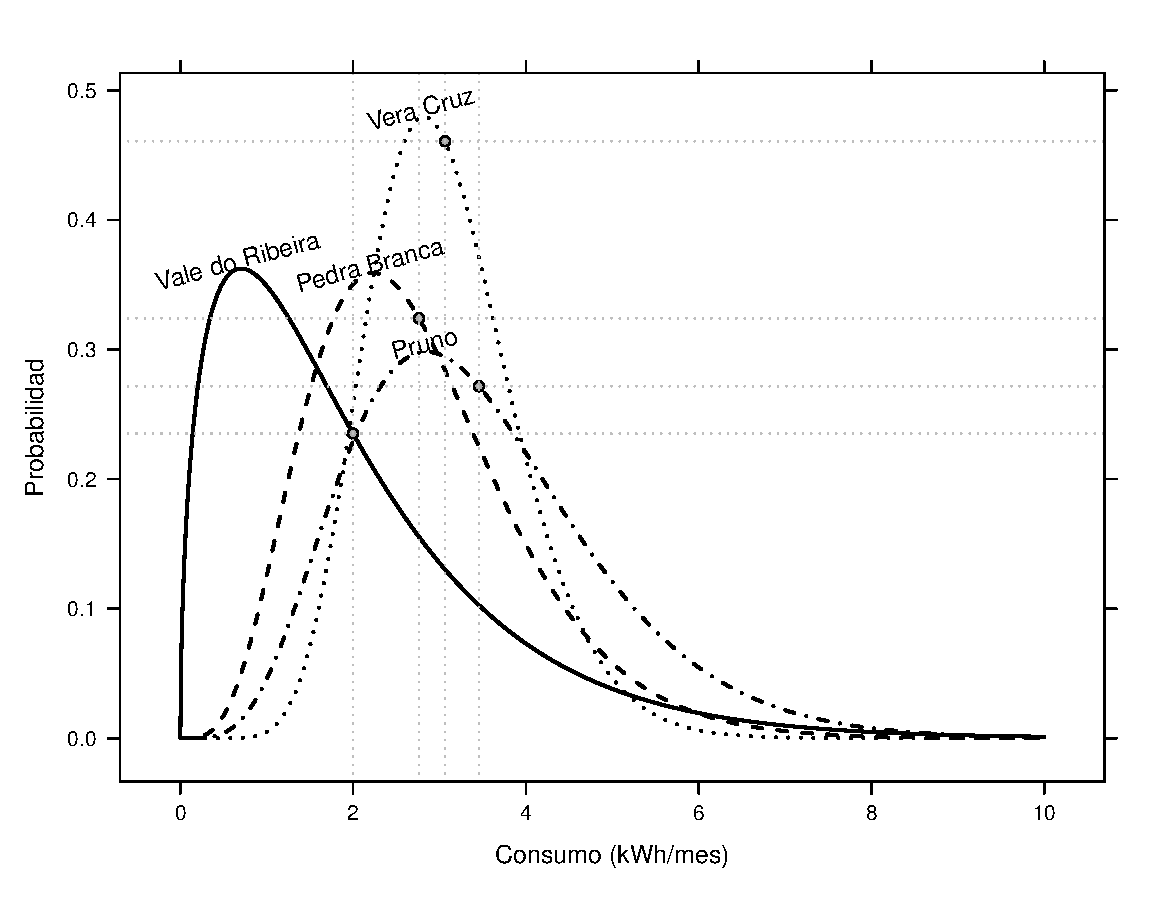
\includegraphics[width=.9\linewidth]{../figs/ConsumoGamma.pdf}
\end{center}
\end{frame}

\begin{frame}[label={sec:orgadb8b8d}]{Relación entre el consumo y la fiabilidad}
\begin{itemize}
\item La variación en el consumo se amplifica en la variación de la LLP.
\item Diseño robusto: funcionamiento en amplio abanico de condiciones (ambientales y humanas).
\end{itemize}
\begin{center}
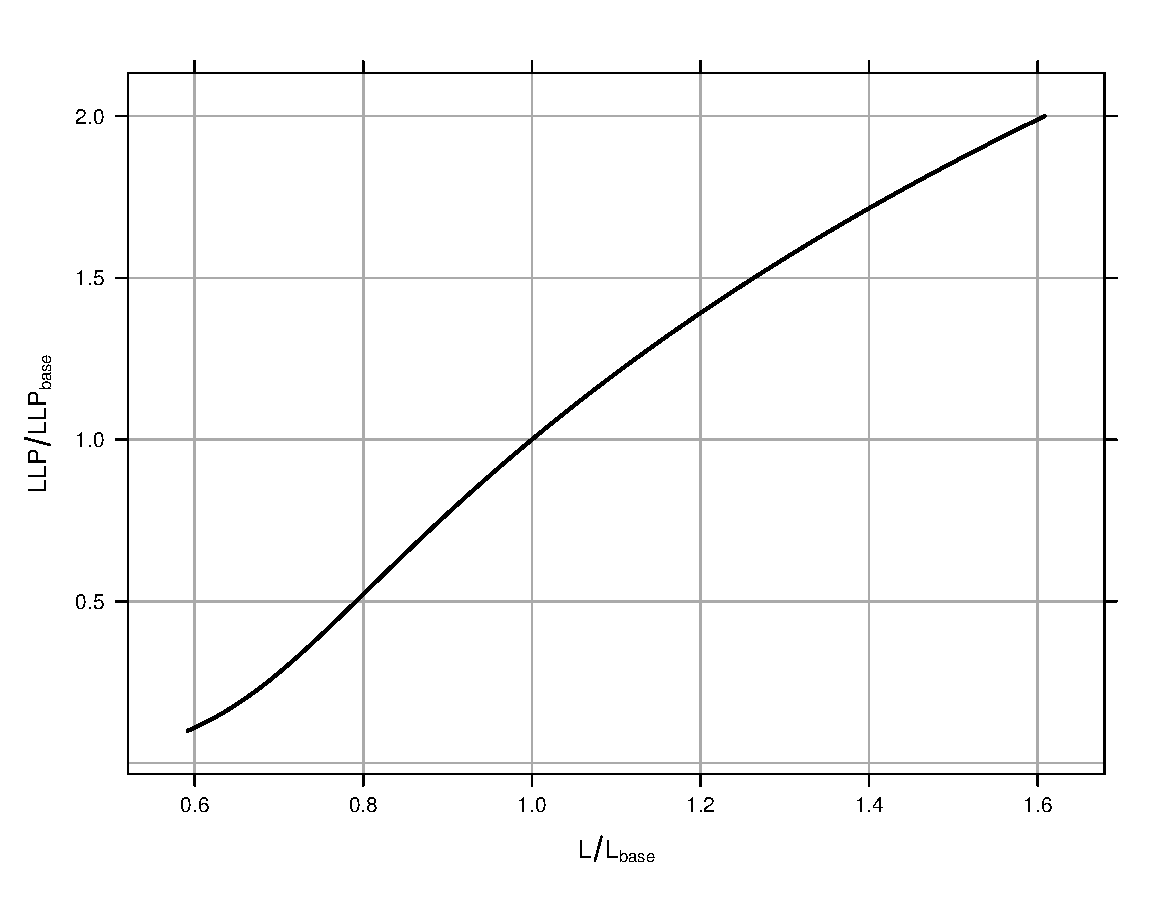
\includegraphics[height=0.7\textheight]{../figs/ConsumoLLP.pdf}
\end{center}
\end{frame}

\subsection{Escenarios de Consumo}
\label{sec:orge5a6fe3}
\begin{frame}[label={sec:org1bfdcab}]{SHS 1}
\begin{block}{120 Wh/dia}
\begin{itemize}
\item Iluminación

\item Radio

\item TV b/n,

\item Sin frigorífico
\end{itemize}
\end{block}

\begin{block}{Valores recomendados}
$$\begin{aligned}
C_{A} & = & 1.1\\
3\leq & C_{s} & \leq5
\end{aligned}$$
\end{block}
\end{frame}

\begin{frame}[label={sec:org7b3d8e3}]{SHS 2}
\begin{block}{250 Wh/dia}
\begin{itemize}
\item Iluminación

\item Radio

\item TV color

\item Sin frigorífico
\end{itemize}
\end{block}

\begin{block}{Valores recomendados}
$$\begin{aligned}
C_{A} & = & 1.1\\
3\leq & C_{s} & \leq5
\end{aligned}$$
\end{block}
\end{frame}

\begin{frame}[label={sec:orgc71c9dc}]{SHS 3}
\begin{block}{1000 Wh/dia}
\begin{itemize}
\item Iluminación

\item radio

\item TV color

\item Con frigorífico eficiente
\end{itemize}
\end{block}

\begin{block}{Valores recomendados}
$$\begin{aligned}
C_{A} & = & 1.1\\
C_{S} & = & 5
\end{aligned}$$
\end{block}
\end{frame}

\begin{frame}[label={sec:orgca77897}]{Centrales}
\begin{block}{}
\begin{itemize}
\item Todo AC

\item 500 Wh/dia por vivienda.
\end{itemize}
\end{block}

\begin{block}{Valores recomendados}
$$\begin{aligned}
C_{A} & = & 1.1\\
C_{S} & = & 5\end{aligned}$$
\end{block}
\end{frame}
\end{document}